\chapter{The Microcanonical Ensemble}\label{ch:b3:microcanonical-ensemble}

A cubic centimetre of air holds $2.5\times10^{19}$ molecules. No
computer will ever integrate their equations of motion, and no
experiment could supply the initial conditions --- yet the gas obeys
laws of splendid simplicity, and the thermodynamics of the Year 1
volume described them without ever mentioning a molecule. This
chapter builds the bridge: \emph{statistical physics}, which derives
the laws of heat from mechanics plus honest counting. The whole
edifice stands on one postulate --- an isolated system is equally
likely to be in any microscopic state compatible with its energy ---
made legitimate by Liouville's theorem
(\cref{ch:b3:hamiltonian-mechanics}) and made powerful by the sheer
size of the numbers: when configurations are counted in units of
$10^{10^{20}}$, ``overwhelmingly probable'' and ``certain'' become
indistinguishable, and probability hardens into law. Out of the
counting come entropy, temperature, pressure and the second law ---
and, at the chapter's end, the reason a rubber band pulls back.

\section{Microstates, macrostates, and the postulate}

\begin{definition}[Microstates and macrostates]\label{def:b3:microcanonical-ensemble:states}
\index{microstate}\index{macrostate}\index{multiplicity}
A \emph{microstate} is a complete microscopic specification of a
system --- every quantum number of every particle (or, classically,
every position and momentum, counted in phase-space cells of $h^3$
per particle, \cref{prop:b3:schrodinger-three-dimensions:counting}).
A \emph{macrostate} is what thermodynamics can see: energy $E$,
volume $V$, particle number $N$, magnetisation\dots\ The
\emph{multiplicity} $\Omega(E, V, N)$ is the number of microstates
wearing the same macrostate.
\end{definition}

\begin{theorem}[The fundamental postulate]\label{thm:b3:microcanonical-ensemble:postulate}
\index{microcanonical ensemble}\index{fundamental postulate}
An isolated system in equilibrium is found with equal probability in
each of its $\Omega(E, V, N)$ accessible \omterm{def:b3:microcanonical-ensemble:states}{microstates}. All of
equilibrium statistical physics follows from this single sentence.
Its credentials: Liouville's theorem shows the uniform distribution
over the energy shell is the one that dynamics preserves --- no flow
ever bunches phase-space probability --- and a century and a half of
consequences have never disagreed with an experiment.
\end{theorem}
\admitted

\begin{example}[A magnet of $N$ coins]\label{ex:b3:microcanonical-ensemble:spins}
$N$ independent spins, each up or down: $2^N$ \omterm{def:b3:microcanonical-ensemble:states}{microstates}. The
\omterm{def:b3:microcanonical-ensemble:states}{macrostate} ``$n$ up'' has \omterm{def:b3:microcanonical-ensemble:states}{multiplicity} $\Omega(n) = \binom Nn$,
overwhelmingly peaked at $n = N/2$ with relative width
$\sim1/\sqrt N$. For $N = 100$: the all-up state is one; the
balanced \omterm{def:b3:microcanonical-ensemble:states}{macrostate} holds $\num{1e29}$. For $N = 10^{20}$,
deviations of even $10^{-8}$ in the up-fraction are suppressed by
factors like $\eu^{-10^4}$: the system \emph{is} at its peak, and
what we call equilibrium is the \omterm{def:b3:microcanonical-ensemble:states}{macrostate} with the most
\omterm{def:b3:microcanonical-ensemble:states}{microstates}.
\end{example}

\begin{omfigure}
\begin{tikzpicture}
  \begin{axis}[omaxis, axis x line=bottom, axis y line=left,
    width=11.4cm, height=5.4cm, xmin=0, xmax=1, ymin=0, ymax=1.15,
    xlabel={fraction of spins up}, ylabel={probability (scaled)},
    xlabel style={at={(axis description cs:0.5,-0.1)}, anchor=north},
    xtick={0.25,0.5,0.75}, ytick=\empty, clip=false,
    legend style={font=\scriptsize, at={(0.03,0.95)}, anchor=north west,
      draw=none, fill=none}]
    \addplot[omExo, thick, domain=0:1, samples=120]
      {exp(-(x-0.5)^2*2*10)};
    \addlegendentry{$N = 10$}
    \addplot[omThm, thick, domain=0:1, samples=200]
      {exp(-(x-0.5)^2*2*100)};
    \addlegendentry{$N = 100$}
    \addplot[omDef, very thick, domain=0.3:0.7, samples=300]
      {exp(-(x-0.5)^2*2*3000)};
    \addlegendentry{$N = 3000$}
  \end{axis}
\end{tikzpicture}

{\small The \omterm{def:b3:microcanonical-ensemble:states}{multiplicity} of the spin system against its up-fraction,
for growing $N$: the peak sharpens as $1/\sqrt N$. At $N \sim
10^{20}$ the ``distribution'' is, for every practical purpose, a
single value --- macroscopic definiteness out of microscopic
democracy.}
\end{omfigure}

\section{Entropy is a count}

\begin{definition}[Boltzmann entropy]\label{def:b3:microcanonical-ensemble:entropy}
\index{entropy!statistical}
The \emph{statistical entropy} of a \omterm{def:b3:microcanonical-ensemble:states}{macrostate} is
\[
S = k_{\text{B}}\ln\Omega , \qquad
k_{\text{B}} = \qty{1.38e-23}{J/K} .
\]
The logarithm makes entropy \emph{additive} where multiplicities
\emph{multiply}: for independent systems $\Omega = \Omega_1\Omega_2$
and $S = S_1 + S_2$; Boltzmann's constant calibrates the count to
the kelvin-and-joule units thermodynamics had already chosen. This
$S$, we will verify, is the entropy of the Year 1 volume's second
law --- now with a microscopic meaning: entropy measures, in
logarithmic currency, \emph{how many ways} the \omterm{def:b3:microcanonical-ensemble:states}{macrostate} can be
realised.
\end{definition}

\begin{proposition}[Entropy of the ideal gas]\label{prop:b3:microcanonical-ensemble:gas}
\index{Sackur--Tetrode formula}
Counting the quantum states of $N$ identical atoms in a box
(\cref{prop:b3:schrodinger-three-dimensions:counting}, one cell of
$h^3$ per atom in \omterm{def:b3:hamiltonian-mechanics:hamiltonian}{phase space}, divided by $N!$ for identity ---
\cref{exo:b3:identical-particles:10}) gives
\[
S = Nk_{\text{B}}\Big[\ln\Big(\frac VN\,\frac1{\lambda_T^3}\Big)
 + \frac52\Big] , \qquad
\lambda_T = \frac{h}{\sqrt{2\pi mk_{\text{B}}T}}
\]
(the \emph{Sackur--Tetrode formula}; $\lambda_T$, the thermal de
Broglie wavelength, is the size of an atom's wave packet at
temperature $T$). Two remarkable audits: the formula is extensive
\emph{only} thanks to the $N!$; and its absolute value --- including
the $h$ --- matches calorimetric entropies of real gases
(\cref{exo:b3:microcanonical-ensemble:11}): classical
thermodynamics, measured in the nineteenth century, already knew
Planck's constant without knowing it.
\end{proposition}
\admitted

\section{Temperature is a derivative of counting}

\begin{theorem}[Equilibrium and temperature]\label{thm:b3:microcanonical-ensemble:temperature}
\index{temperature!statistical definition}
Let two systems exchange energy, the total $E = E_1 + E_2$ fixed.
The joint \omterm{def:b3:microcanonical-ensemble:states}{multiplicity} $\Omega_1(E_1)\,\Omega_2(E - E_1)$ is
maximal --- overwhelmingly so --- at the partition where
\[
\frac{\partial S_1}{\partial E_1} =
\frac{\partial S_2}{\partial E_2} .
\]
Defining
\[
\frac1T = \frac{\partial S}{\partial E}\bigg|_{V,N} ,
\]
equilibrium is \emph{equality of temperature}, and energy flows
spontaneously from high $T$ to low $T$ because that direction
increases the total count. The same logic applied to volume and
particle exchange yields $P/T = \partial S/\partial V$ and $-\mu/T
= \partial S/\partial N$: all of thermodynamics' intensive
quantities are derivatives of the count.
\end{theorem}

\begin{proof}
Maximise $\ln\Omega_1 + \ln\Omega_2$ over $E_1$: the stationarity
condition is the stated equality. Sharpness: the peak's width is
$\sim E/\sqrt N$ (\cref{exo:b3:microcanonical-ensemble:7}), so the
maximum is the observed state. If $\partial S_1/\partial E_1 >
\partial S_2/\partial E_2$, moving energy \emph{into} 1 raises
$S_{\text{tot}}$: the colder body (larger $\partial S/\partial E$)
absorbs --- heat flows hot to cold as a counting statement. Check
on the ideal gas: $S \propto \tfrac32 Nk_{\text{B}}\ln E + \cdots$
gives $1/T = \tfrac32 Nk_{\text{B}}/E$, i.e.\ $E = \tfrac32
Nk_{\text{B}}T$ --- the kinetic-theory result of the Year 1 volume,
recovered from pure counting.
\end{proof}

\begin{omfigure}
\begin{tikzpicture}
  \begin{axis}[omaxis, axis x line=bottom, axis y line=left,
    width=11.2cm, height=5.2cm, xmin=0, xmax=1, ymin=0, ymax=1.2,
    xlabel={share of the energy in system 1},
    ylabel={$\Omega_1\Omega_2$ (scaled)},
    xlabel style={at={(axis description cs:0.5,-0.1)}, anchor=north},
    xtick={0.4}, xticklabels={$E_1^{\text{eq}}$}, ytick=\empty, clip=false]
    \addplot[omDef, very thick, domain=0:1, samples=250]
      {exp(-(x-0.4)^2*900)};
    \node[omDef, font=\scriptsize, anchor=west] at (axis cs:0.47,0.75)
      {width $\sim 1/\sqrt N$};
  \end{axis}
\end{tikzpicture}

{\small Two systems sharing energy: the joint count against the
split. The equilibrium partition --- equal temperatures --- is not
merely the likeliest; for macroscopic $N$ it is the only one ever
observed.}
\end{omfigure}

\section{The second law, and stranger things}

\begin{proposition}[Irreversibility is arithmetic]\label{prop:b3:microcanonical-ensemble:second-law}
\index{second law!statistical}
A \omterm{def:b3:lagrangian-mechanics:coordinates}{constraint} released (a wall removed, a valve opened) can only
enlarge the accessible count: $\Omega$ grows, $S$ grows --- the
second law of the Year 1 volume, now as a statement about
probability. Reversals are not forbidden but \emph{discounted}: a
gas of $N$ molecules re-gathering into the left half has probability
$2^{-N}$, and for one cubic centimetre of air the waiting time
exceeds the age of the universe by a factor with $10^{19}$ digits.
The arrow of time, at this level, is the direction in which counts
increase.
\end{proposition}

\begin{proof}[Partial proof]
Removing a \omterm{def:b3:lagrangian-mechanics:coordinates}{constraint} makes every formerly accessible \omterm{def:b3:microcanonical-ensemble:states}{microstate}
still accessible and adds new ones: $\Omega$ cannot decrease. The
free-expansion count: each molecule doubles its accessible volume,
$\Omega \to 2^N\Omega$, so $\Delta S = Nk_{\text{B}}\ln2$ ---
exactly the thermodynamic result for isothermal free doubling.
\end{proof}

\begin{example}[Negative temperature]\label{ex:b3:microcanonical-ensemble:negative}
\index{negative temperature}
A system whose energy is \emph{bounded above} --- $N$ spins in a
field, energy from $-N\epsilon$ to $+N\epsilon$ --- has $\Omega(E)$
rising then \emph{falling}: beyond the balanced point, adding energy
reduces the count. There $\partial S/\partial E < 0$: the
temperature is \emph{negative}. Such states exist (population
inversions --- the working state of every laser medium --- and
spin systems prepared by field reversal) and they are not cold but
\emph{hotter than every positive temperature}: energy flows from any
$T < 0$ body into any $T > 0$ body. The honest ordering of
temperatures runs $+0, \dots, +\infty \equiv -\infty, \dots, -0$:
what $1/T$ orders naturally, $T$ garbles
(\cref{exo:b3:microcanonical-ensemble:9}).
\end{example}

\begin{omfigure}
\begin{tikzpicture}
  \begin{axis}[omaxis, axis x line=bottom, axis y line=left,
    width=10.8cm, height=5.4cm, xmin=-1.05, xmax=1.05, ymin=0, ymax=0.78,
    xlabel={$E/N\epsilon$}, ylabel={$S/Nk_{\text{B}}$},
    xlabel style={at={(axis description cs:0.5,-0.1)}, anchor=north},
    xtick={-1,0,1}, ytick=\empty, clip=false]
    \addplot[omDef, very thick, domain=-0.999:0.999, samples=250]
      {-0.5*(1+x)*ln(0.5*(1+x)) - 0.5*(1-x)*ln(0.5*(1-x))};
    \node[font=\scriptsize, anchor=south] at (axis cs:-0.62,0.6)
      {$\partial S/\partial E > 0$: $T > 0$};
    \node[font=\scriptsize, anchor=south] at (axis cs:0.62,0.6)
      {$\partial S/\partial E < 0$: $T < 0$};
    \draw[gray, dashed] (axis cs:0,0) -- (axis cs:0,0.7);
    \node[font=\scriptsize, anchor=south] at (axis cs:0,0.71) {$T = \pm\infty$};
  \end{axis}
\end{tikzpicture}

{\small Entropy of the two-level spin system against energy. On the
rising flank temperature is positive; at the crest it passes through
infinity; on the falling flank --- population inverted --- it is
negative, and hotter than anything on the left.}
\end{omfigure}

\begin{method}[Microcanonical craft]\label{met:b3:microcanonical-ensemble:method}
(1) Enumerate: what is a \omterm{def:b3:microcanonical-ensemble:states}{microstate} here, and what does the
\omterm{def:b3:microcanonical-ensemble:states}{macrostate} fix? (2) Count $\Omega$ --- combinatorics for discrete
units, phase-space volume over $h^{3N}N!$ for gases. (3) Take the
logarithm early: Stirling ($\ln N! \approx N\ln N - N$) turns
products into tractable sums. (4) Differentiate $S$: energy
derivative for $T$, volume for $P$, number for $\mu$; length or
magnetisation derivatives for tensions and fields
(\cref{pb:b3:microcanonical-ensemble:1}). (5) Trust the peak:
fluctuations are down by $1/\sqrt N$, so replace ``most probable''
by ``equals'' and apologise to no one.
\end{method}

\begin{omfigure}
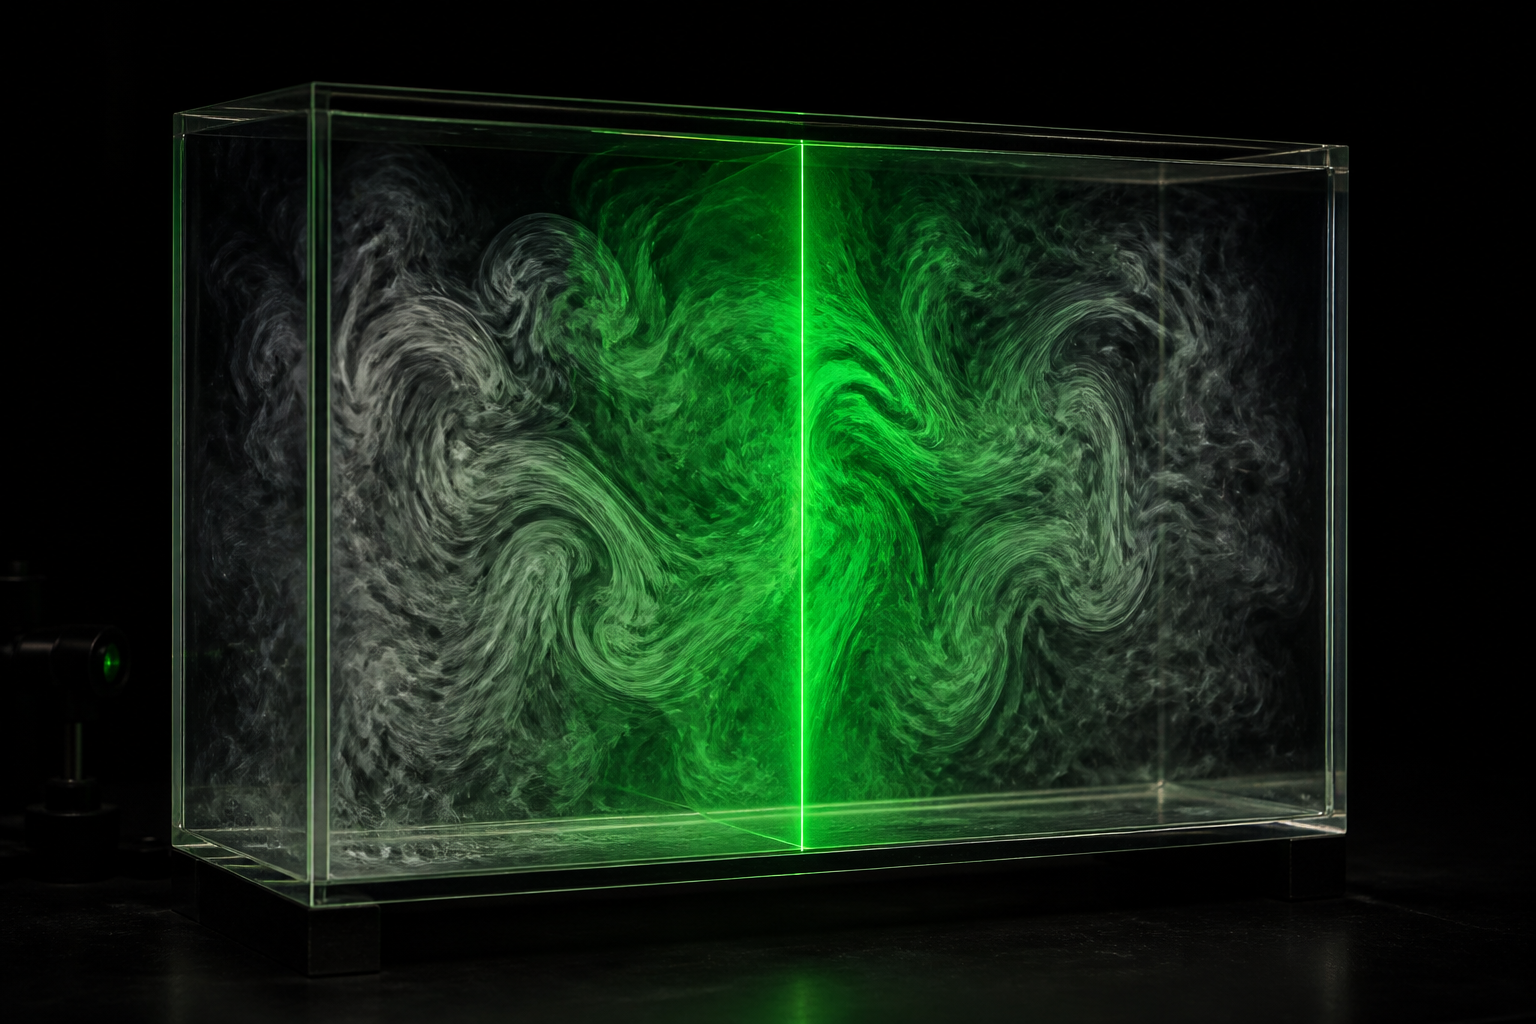
\includegraphics[width=0.58\linewidth]{images/book5/ai/b5-16-laser-sheet-smoke.png}

{\small Smoke stirred in a box, cut by a laser sheet: micro-motion beyond any bookkeeping, statistics taking over --- the moment a mechanics problem becomes an entropy problem.}
\end{omfigure}

\section{Exercises}

\begin{exercise}[$\star$]\label{exo:b3:microcanonical-ensemble:1}
Four spins. (a) List the multiplicities $\Omega(n)$ of the
\omterm{def:b3:microcanonical-ensemble:states}{macrostates} ``$n$ up''. (b) The probability of each \omterm{def:b3:microcanonical-ensemble:states}{macrostate} under
the postulate. (c) The entropy (in units of $k_{\text{B}}$) of each.
(d) Which \omterm{def:b3:microcanonical-ensemble:states}{macrostate} is ``equilibrium'', and how bad an
approximation is ``the system is surely there'' at $N = 4$?
\end{exercise}

\begin{exercise}[$\star$]\label{exo:b3:microcanonical-ensemble:2}
Stirling in practice. (a) Compare $\ln N!$ with $N\ln N - N$ for
$N = 10$ and $N = 100$ (use $\ln10! = 15.10$, $\ln100! = 363.7$).
(b) Show the relative error falls like $\ln N/N$. (c) Use Stirling
to show $\ln\binom N{N/2} \approx N\ln2 - \tfrac12\ln N + $ const.
(d) Why is dropping the $\tfrac12\ln N$ utterly safe in a mole?
\end{exercise}

\begin{exercise}[$\star$]\label{exo:b3:microcanonical-ensemble:3}
(a) Show that for two independent systems $S = S_1 + S_2$. (b) A
system's $\Omega$ doubles: by how much does $S$ rise --- and what
physical act (\cref{prop:b3:microcanonical-ensemble:second-law})
does that correspond to for one particle? (c) Compute the entropy,
in $k_{\text{B}}$ and in J/K, of a shuffled deck of 52 cards
($\ln52! \approx 156.4$). (d) Why is card entropy thermodynamically
negligible while molecular entropy is not?
\end{exercise}

\begin{exercise}[$\star$]\label{exo:b3:microcanonical-ensemble:4}
Free expansion, audited. One mole doubles its volume into vacuum.
(a) $\Delta S$ from the counting argument. (b) The probability of
observing the gas back in the original half. (c) Estimate the time
scale for such a fluctuation given molecular rearrangement times of
\qty{e-10}{s} --- and compare with the age of the universe
(\qty{4e17}{s}). (d) In what precise sense is the second law
``only'' probabilistic?
\end{exercise}

\begin{exercise}[$\star\star$]\label{exo:b3:microcanonical-ensemble:5}
Ideal-gas counting. Starting from
$\Omega \propto \dfrac{V^N}{N!\,h^{3N}}\times$ (momentum-shell
volume $\propto E^{3N/2}$): (a) show $S = Nk_{\text{B}}[\ln V +
\tfrac32\ln E] - k_{\text{B}}\ln N! + $ const. (b) Show that
without the $N!$, doubling the system (both $V$ and $N$) would
\emph{not} double $S$ --- the extensivity failure of
\cref{exo:b3:identical-particles:10}. (c) With Stirling, put the
result in the form $S = Nk_{\text{B}}[\ln(V/N) + \tfrac32\ln(E/N)]
+ $ const$\cdot N$. (d) Which physical inputs fixed the two
``consts'' history left undetermined (quantum cell size; particle
identity)?
\end{exercise}

\begin{exercise}[$\star\star$]\label{exo:b3:microcanonical-ensemble:6}
Thermodynamics from derivatives. Using the form of
\cref{exo:b3:microcanonical-ensemble:5}(c): (a) compute $1/T =
\partial S/\partial E$ and recover $E = \tfrac32 Nk_{\text{B}}T$;
(b) compute $P/T = \partial S/\partial V$ and recover $PV =
Nk_{\text{B}}T$; (c) derive the \omterm{prop:b3:hamiltonian-mechanics:adiabatic}{adiabatic invariant}: at constant
$S$ and $N$, show $VE^{3/2}$ is fixed, i.e.\ $TV^{2/3}$ --- and
match to the $PV^{5/3}$ of the Year 1 volume; (d) state what has
been achieved: which empirical laws just became theorems of
counting.
\end{exercise}

\begin{exercise}[$\star\star$]\label{exo:b3:microcanonical-ensemble:7}
Sharpness of equilibrium. Two equal ideal-gas blocks share total
energy $E$. (a) Show $\ln[\Omega_1\Omega_2]$ is maximal at the
even split. (b) Expand to second order in the imbalance $x =
(E_1 - E_2)/E$ and show the probability is
$\propto\eu^{-3Nx^2/4}$ (each block $\tfrac32 N$ \omterm{def:b3:lagrangian-mechanics:coordinates}{degrees of
freedom} --- keep factors loose). (c) For $N = 10^{22}$: the
r.m.s.\ imbalance. (d) The temperature difference that imbalance
represents, for gas at \qty{300}{K}: could any thermometer see
it?
\end{exercise}

\begin{exercise}[$\star\star$]\label{exo:b3:microcanonical-ensemble:8}
The two-level (Schottky) solid: $N$ sites, each of energy $0$ or
$\epsilon$; $n$ excited. (a) $\Omega(n)$ and $S(n)$. (b) With $E =
n\epsilon$ and Stirling, derive
\[
\frac1T = \frac{k_{\text{B}}}{\epsilon}\,
\ln\frac{N - n}{n} ,
\qquad\text{hence}\qquad
\frac nN = \frac{1}{\eu^{\epsilon/k_{\text{B}}T} + 1} .
\]
(c) Sketch $E(T)$ and the heat capacity: a bump (the
\emph{Schottky anomaly}) near $k_{\text{B}}T \sim \epsilon/2$ ---
why does $C$ vanish at both ends? (d) Where has the occupation
formula's shape appeared before, and where will it return
(\cref{ch:b3:quantum-statistics})?
\end{exercise}

\begin{exercise}[$\star\star$]\label{exo:b3:microcanonical-ensemble:9}
Below zero. For the spin system of
\cref{ex:b3:microcanonical-ensemble:negative} with level splitting
$\epsilon$: (a) show $T < 0$ exactly when more than half the spins
are up (population inverted). (b) Compute $T$ for a 60:40 inversion
with $\epsilon = \qty{e-4}{eV}$. (c) Show energy always flows from
negative-$T$ to positive-$T$ bodies (compare $\partial
S/\partial E$). (d) Why can a system with unbounded energy (a gas)
never reach $T < 0$?
\end{exercise}

\begin{exercise}[$\star\star\star$]\label{exo:b3:microcanonical-ensemble:10}
Mixing, quantitatively. Two different gases ($N$ each, volumes $V$)
are joined. (a) Compute $\Delta S$ by counting. (b) Same gas:
show, $N!$'s included, $\Delta S = 0$. (c) Helium-3 and helium-4
are different: joining them \emph{does} create $2Nk_{\text{B}}\ln2$
--- yet no heat flows and no work is done: where is the entropy
increase physically (what would separating them again cost)? (d)
The minimum work to re-separate at temperature $T$: express it, and
name the modern industry built on paying it (isotope separation).
\end{exercise}

\begin{exercise}[$\star\star\star$]\label{exo:b3:microcanonical-ensemble:11}
The tables knew about $h$. Sackur--Tetrode for argon ($m =
\qty{6.6e-26}{kg}$) at \qty{300}{K}, \qty{1}{bar} ($V/N =
k_{\text{B}}T/P$): (a) compute $\lambda_T$; (b) compute $S/N
k_{\text{B}}$; (c) compare with the calorimetric value
$S_{\text{molar}} = \qty{154.8}{J/(mol.K)}$, i.e.\ $S/Nk_{\text{B}}
= 18.6$; (d) explain what is being tested: which two quantum
inputs sit inside a number measured with ice calorimeters before
1912?
\end{exercise}

\begin{exercise}[$\star\star\star$]\label{exo:b3:microcanonical-ensemble:12}
Fluctuations you can see. The number of molecules in a small volume
$v$ of gas fluctuates; the probability of a relative deviation
$\delta$ is $\propto\eu^{-\bar n\delta^2/2}$ ($\bar n = Nv/V$ ---
accept this Gaussian, or derive from the binomial). (a) For $v$ a
cube of side \qty{550}{nm} at atmospheric density: $\bar n$ and
the r.m.s.\ $\delta$. (b) Why are these permanent few-per-mille
density ripples at optical scales exactly what
\cref{pb:b3:perturbation-theory:1} needed to let air scatter at
all? (c) At what $\bar n$ (hence what scale) would fluctuations
reach $10\%$? (d) Close the loop in one sentence: the blue of the
sky is a statement about $\sqrt N$ statistics.
\end{exercise}

\section{Problem: The entropic spring}

\begin{problem}[{Weekend problem --- why rubber pulls back}]\label{pb:b3:microcanonical-ensemble:1}
Stretch a rubber band and it snaps back --- yet its molecules'
bonds are barely deformed and its internal energy barely changes.
Rubber's restoring force is not energy seeking a minimum but
\emph{entropy seeking a maximum}: the first great victory of pure
counting over mechanism, with the same mathematics running today's
single-molecule DNA experiments. Model: a chain of $N$ rigid links,
each of length $b$, each pointing left or right along the pull
axis; end-to-end extension $x = (n_+ - n_-)\,b$.

\medskip\noindent\textbf{Part I --- Counting configurations.}
\begin{enumerate}
  \item Express $n_\pm$ in terms of $N$ and $x$, and write the
        \omterm{def:b3:microcanonical-ensemble:states}{multiplicity} $\Omega(x)$.
  \item Where is $\Omega$ maximal, and what does that say about a
        free chain's preferred extension?
  \item With Stirling, show for $x \ll Nb$:
        \[
        S(x) \approx S(0) - \frac{k_{\text{B}}x^2}{2Nb^2} .
        \]
  \item The chain's energy is (in this model) independent of $x$:
        justify calling any restoring force ``entropic''.
  \item The r.m.s.\ extension of the free chain is $b\sqrt N$
        (random walk): for $N = 10^4$ and $b = \qty{0.5}{nm}$,
        compare the coil size with the stretched length $Nb$.
  \item Real rubber is a network of such chains between
        cross-links: which single parameter of the model does
        vulcanisation (more cross-links) change?
\end{enumerate}

\medskip\noindent\textbf{Part II --- The force of counting.}
\begin{enumerate}[resume]
  \item For a system held at temperature $T$, the tension required
        to hold extension $x$ is $f = -T\,\partial S/\partial x$
        (accept this from $\dd E = T\dd S + f\dd x$ at constant
        energy): derive
        \[
        f = \frac{k_{\text{B}}T\,x}{Nb^2} .
        \]
  \item \omterm{thm:b3:continuum-elasticity:hooke}{Hooke's law} has emerged with spring constant $k =
        k_{\text{B}}T/Nb^2$: evaluate it for one chain with $N =
        \num{e4}$, $b = \qty{0.5}{nm}$ at \qty{300}{K}.
  \item The startling factor is $T$: what should a rubber band
        under fixed load do when \emph{heated}? Contrast with a
        steel spring.
  \item Estimate the force to stretch one chain to half its full
        length, and the force scale $k_{\text{B}}T/b$ at which the
        linear model fails.
  \item A rubber band of \omterm{def:b3:scattering-theory:cross-section}{cross-section} \qty{1}{mm^2} contains
        $\sim\num{e14}$ effective chains in parallel: estimate its
        spring constant and compare with experience.
  \item Why does rubber stiffen (not soften) with temperature,
        gram for gram, while metals soften?
\end{enumerate}

\medskip\noindent\textbf{Part III --- The Gough--Joule kitchen.}
\begin{enumerate}[resume]
  \item Stretch a rubber band quickly (adiabatically) against your
        lip: it warms. Explain with the entropy budget: stretching
        \emph{reduces} configurational entropy, so where must
        entropy (heat) go at constant total?
  \item Release it quickly: it cools. Complete the symmetric
        argument.
  \item A weighted rubber band is gently heated (hair dryer): which
        way does the weight move, and why is this the clean
        signature of entropic elasticity?
  \item Design the counter-experiment with a steel spring: what
        happens instead, and why (which kind of elasticity)?
  \item An engine: a wheel with rubber spokes, heated on one side,
        turns steadily. Trace one cycle's logic (heated spokes
        contract, unbalancing the wheel).
  \item The same $f = k_{\text{B}}Tx/Nb^2$ law, measured by
        optical tweezers on single DNA molecules (with $b \approx
        \qty{100}{nm}$, $N \approx 500$ for a bacterial genome
        fragment), gives forces in which range? (Compute
        $k_{\text{B}}T/b$.) Why did this make the model
        \emph{directly} testable on one molecule?
\end{enumerate}

\medskip\noindent\textbf{Part IV --- The moral.}
\begin{enumerate}[resume]
  \item The chain model has no interactions and no energy scale,
        yet produces a force law: state precisely where the force
        ``comes from'' in the microcanonical language of this
        chapter.
  \item Why does the force vanish at $T = 0$ --- and what does
        that say about the nature of elasticity in a world without
        thermal agitation?
  \item Compare the entropic spring constant's $T$-linearity with
        the ideal-gas pressure's $T$-linearity: show both are the
        same phenomenon (counting configurations against a
        \omterm{def:b3:lagrangian-mechanics:coordinates}{constraint}) in different clothes.
  \item The heated band lifts a weight, doing real work: trace
        the energy's source and route (heat in from the dryer,
        entropy bookkeeping, work out) and confirm the first law
        is untouched.
  \item The ideal chain ignores self-avoidance and link-bending
        energy: name one measured feature of real rubber each
        omission hides (sharp stiffening near full extension;
        strain-induced crystallisation and hysteresis).
  \item Proteins fold, membranes flicker, polymers coil: why is
        $k_{\text{B}}T$ at body temperature the natural force
        currency ($k_{\text{B}}T/\unit{nm}$ in piconewtons ---
        compute it) of all soft and living matter?
  \item Summarise the named result: a chain of $10^4$ blind links,
        counted honestly, yields \omterm{thm:b3:continuum-elasticity:hooke}{Hooke's law} with $k =
        k_{\text{B}}T/Nb^2$, predicts that rubber warms when
        stretched and lifts weights when heated --- entropy acting
        as a force, verified from bicycle inner tubes to single
        DNA molecules at $\sim\qty{0.04}{pN}$ scales.
\end{enumerate}
\end{problem}
